% ============================================================
% CAPÍTULO 3: METODOLOGÍA
% ============================================================

\chapter{Metodología}
\label{chap:metodologia}

A continuación se detallan los métodos que se han seguido para la descarga, preprocesamiento
de las señales, extracción de características de variabilidad de ritmo cardíaco  (HRV),
y las arquitecturas de las redes neuronales utilizadas para la predicción de
Fibrilación Auricular a partir de segmentos de ECG en ritmo sinusal.

\section{Descarga y lectura de bases de datos}
\label{sec:descarga}

La descarga de bases de datos se ha realizado desde el Clúster del Instituto de Investigación en
Ingeniería de Aragón (I3A)\footnote{\url{https://i3a.unizar.es/es}}, en concreto, en el grupo de investigación BSICoS\footnote{\url{https://bsicos.i3a.es/}},
utilizando el gestor de descargas \texttt{wget}.

Para la lectura, se ha utilizado la librería \texttt{wfdb} de Python,
que permite leer los registros ECG y extraer las anotaciones correspondientes.
Puesto que el trabajo se centra en la predicción inminente, se han extraido ventanas
inmediatamente anteriores a los episodios de fibrilación auricular (Pre-PAF), en concreto,
de un máximo de 5 minutos anteriores al episodio, además de segmentos de control de ritmo sinusal estable.

Cada registro se ha cargado en memoria como un array de \texttt{NumPy} para su posterior procesamiento.


\section{Preprocesamiento}
\label{sec:preprocesamiento}

El preprocesamiento es esencial por varias razones: las bases de datos utilizadas no
presentan la misma frecuencia de muestreo, ni están medidas con el mismo equipo, por tanto
hay que implementar un pipeline que unifique las características para que los modelos puedan generalizar correctamente.
El pipeline de preprocesamiento consta de tres pasos principales:

\begin{enumerate}
  \item \textbf{Armonización de Canales y Frecuencia de Muestreo:}
  Se unifican todas las señales a exactamente dos canales y una frecuencia de
  muestreo de $128$~Hz. Si un registro tiene menos de dos canales, se realiza un relleno
  (padding) con ceros, si tiene más, se seleccionan únicamente las dos primeras
  derivaciones. En nuestro caso todas las bases de datos contienen 2 canales, pero se comprueba
  por generalidad, para tener la posibilidad de añadir posteriormente bases de datos adicionales.
  El remuestreo se ejecuta mediante interpolación trigonométrica.
  \item \textbf{Atenuación del Ruido e Interferencia:}
  La tarea de la eliminación del ruido se delega a las primeras capas convolucionales de los moedlos,
  que aprenderán los filtros necesarios para su correcta eliminación, optimizados para la tarea.
  \item \textbf{Normalización Z-score Local:}
  Para evitar sesgos debido a las variaciones inter-sujeto o inter-dispositivo en la
  amplitud absoluta de las señales, cada segmento se normaliza de forma independiente
  por canal en el dataloader aplicando:
  \begin{equation}
  x_{\text{norm}} = \frac{x - \mu}{\sigma + 10^{-8}}
  \end{equation}
  donde $\mu$ y $\sigma$ representan la media y desviación estándar de la amplitud
  de cada ventana.
\end{enumerate}


\section{Extracción de Ventanas y Prevención de Data Leakage}
\label{sec:extraccion_ventanas}

Los dos tipos de
segmentos requeridos para la clasificación binaria son:

\begin{itemize}
  \item \textbf{Clase 1 (Pre-PAF):}
  Esta clase representa el estado inmediatamente anterior a un episodio de fibrilación auricular. Se ha optado por extraer
  ventanas de longitud variable, de entre $60$ ($1$ minuto) y $300$ ($5$ minutos) segundos, que parten desde el inicio del episodio
  y retroceden en el timepo hasta 5 minutos, o hasta encontrarse con el inicio de otro episodio. De esta manera, se garantiza
  que el segmento contenga solamente ritmo sinusal.

  \item \textbf{Clase 0 (Normal/Control):}
  Se extraen segmentos estables de ritmo sinusal
  de $5$ minutos de duración, que se encuentren alejados al menos $30$ minutos
  ($1800$ segundos) de cualquier episodio
  (tanto antes como después), para evitar zonas de transición.

  Esto es importante, ya que estamos extrayendo ventanas de clase normal de pacientes 
  tanto con PAF como sanos.

  Esta estrategia es fundamental.
  Si la Clase 0 se compusiera solo de individuos sanos, los modelos aprenderían a identificar
  diferencias morfológicas asociadas a la cardiopatía estructural del paciente, en lugar de identificar
  los cambios transitorios que desencadenan el episodio.

\end{itemize}

Para evitar la filtración de datos (\textit{data leakage}), los segmentos se agrupan estrictamente por sujeto.
Esto garantiza que en validación y test no haya pacientes que ya hayan aparecido en
el entrenamiento, ya que el modelo podría aprender a reconocer la morfología de un paciente concreto en lugar de
aprender a generalizar la predicción de la fibrilación auricular.


\section{Aumento de Datos (Data Augmentation)}
\label{sec:aumentacion}

Debido a que los modelos escalan mejor con grandes cantidades de datos, se ha 
implementado un pipeline de aumento de datos, que aplica modificaciones realistas a las
señales directamente en el dataloader con una probabilidad
del $50\%$ para cada una:
\begin{itemize}
  \item \textbf{Deriva de la Línea de Base (\textit{Baseline Wander}):} Se simula la deriva lenta causada por la respiración del paciente sumando una señal sinusoidal:
  \begin{equation}
  x_{\text{aug}}(t) = x(t) + A \cdot \sin(2\pi \cdot f \cdot t)
  \end{equation}
  donde la frecuencia $f$ se muestrea de manera uniforme en $[0.1, 0.5]$~Hz y la amplitud $A$ en $[0.05, 0.2]$.
  \item \textbf{Ruido Gaussiano Aditivo:} Se simula el ruido instrumental sumando ruido blanco gaussiano con una desviación estándar variable $\sigma_{\text{noise}} \sim U(0.01, 0.05)$.
  \item \textbf{Escalado Aleatorio:} Se multiplica el segmento por un factor de escala $s \sim U(0.85, 1.15)$ para simular fluctuaciones en la ganancia del amplificador.
  \item \textbf{Slice Aleatorio de Ventana:} Dado que las redes se entrenan con ventanas
  de $60$ segundos, y contamos con señales de hasta 5 minutos, se extraen 60 segundos aleatorios.
  En validación y test, se toma de forma determinista los últimos $60$ segundos
  (el instante más cercano al inicio de la crisis en la Clase 1).
\end{itemize}

En la figura~\ref{fig:data_augmentation_demo} se ilustra una demostración visual del efecto individual y
combinado de estas técnicas de aumentación de datos aplicadas a un segmento real de electrocardiograma.

\begin{figure}[htbp]
  \centering
  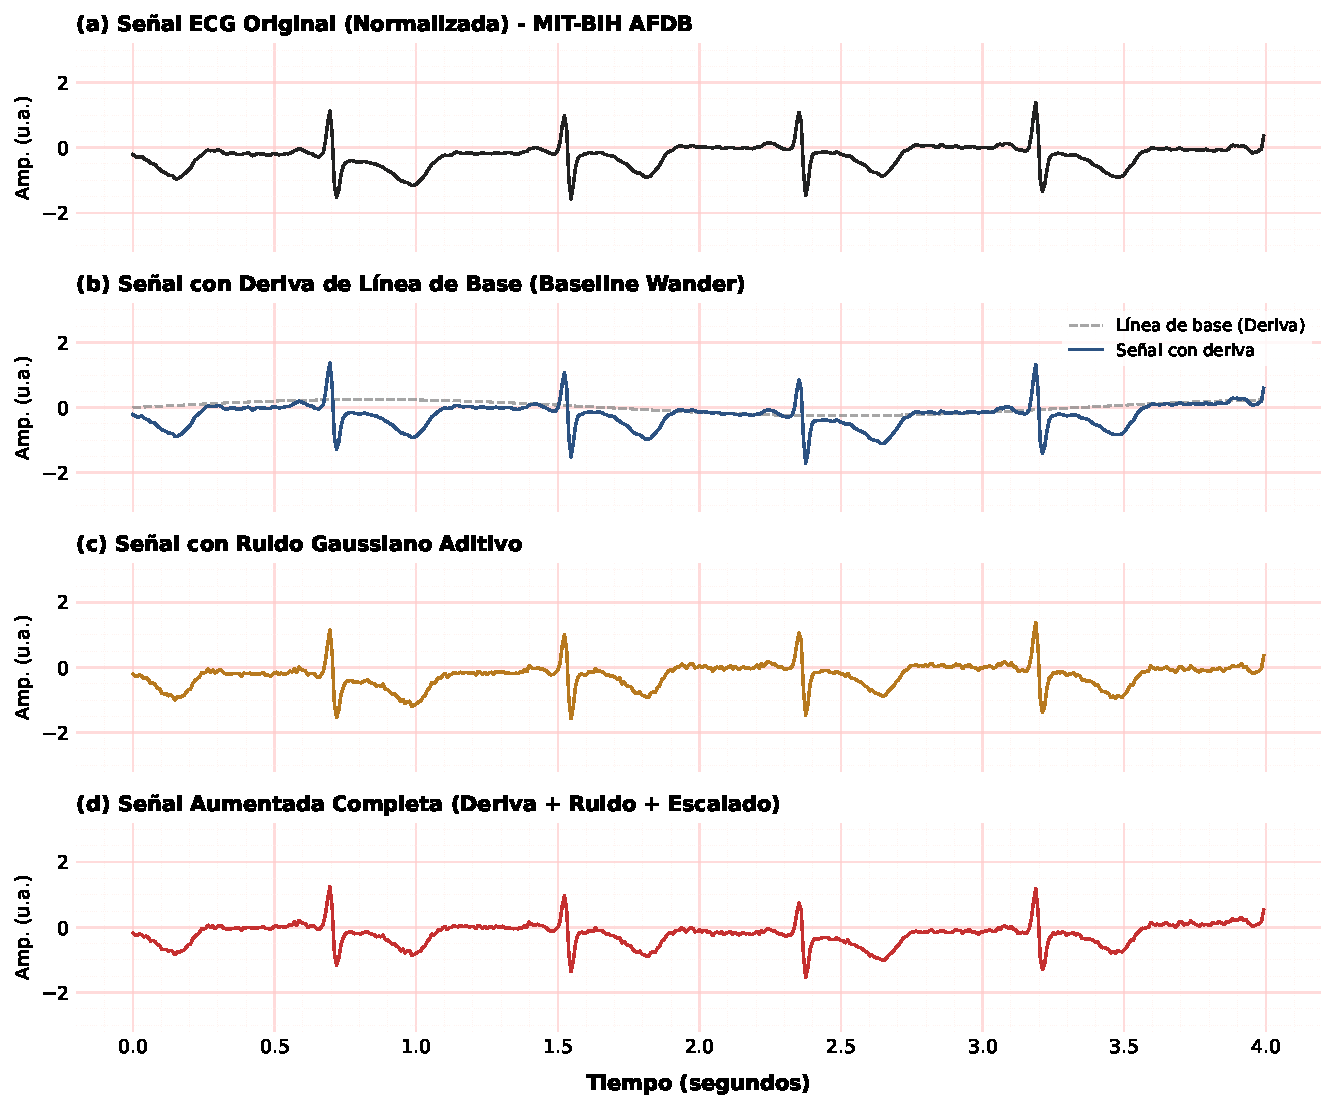
\includegraphics[width=0.9\textwidth]{img/data_augmentation_demo.pdf}
  \caption{Efecto del aumento de datos sobre un segmento de ECG de 4 segundos. Se muestra (a) la señal original
normalizada, (b) la adición de deriva lenta (baseline wander), (c) la adición de ruido de alta frecuencia, y (d) el
resultado combinado de todas las transformaciones.}
  \label{fig:data_augmentation_demo}
\end{figure}

\section{Extracción de Variabilidad del Ritmo Cardíaco (HRV)}
\label{sec:hrv}

Como información complementaria, se calculan nueve variables de variabilidad de ritmo cardíaco (HRV)
a partir de las anotaciones de los picos QRS procedentes de las bases de datos, utilizando las ventanas
de ritmo sinusal de 5 minutos. (Reescalados a $128$~Hz)

\begin{itemize}
      \item \textbf{Métricas Temporales:}
      \begin{itemize}
          \item \textit{Media de intervalos RR} (\texttt{mean\_rr}): Promedio aritmético de los intervalos, expresado en segundos.
          \item \textit{Desviación estándar de intervalos RR} (\texttt{std\_rr}): Medida de la variabilidad global del registro.
          \item \textit{RMSSD} (\texttt{rmssd}): Raíz cuadrada de la media de las diferencias al cuadrado de intervalos sucesivos:
          \begin{equation}
              \text{RMSSD} = \sqrt{\frac{1}{N-1} \sum_{i=1}^{N-1} (RR_{i+1} - RR_i)^2}
          \end{equation}
          \item \textit{pNN50} (\texttt{pnn50}): Porcentaje de intervalos sucesivos que difieren en más
          de $50\text{ ms}$:
          \begin{equation}
              NN50 = \text{Número de intervalos } i \text{ tales que } |RR_{i+1} - RR_i| > 0.05\text{ s}
          \end{equation}
          \begin{equation}
              pNN50 = \frac{NN50}{N - 1} \times 100
          \end{equation}
          donde $N$ representa el número de intervalos $RR$ totales analizados en el segmento.
          \item \textit{Frecuencia cardíaca instantánea} (\texttt{mean\_hr} y \texttt{std\_hr}):
          Obtenida para cada intervalo mediante $\text{HR}_i = 60 / RR_i$
          y calculando su media y desviación estándar.
      \end{itemize}

      \item \textbf{Métricas Frecuenciales:}
      Dado que la serie de intervalos $RR$ es una señal discreta de frecuencia de muestreo no uniforme debido
      a que depende de cada latido, se requiere un preprocesamiento para estimar la Densidad Espectral
      de Potencia (PSD):
      \begin{itemize}
          \item \textit{Interpolación y Remuestreo:} A partir de la serie temporal acumulada de los
          intervalos $RR$, se realiza una interpolación lineal y un remuestreo uniforme a una frecuencia
          fija de $4\text{ Hz}$ para que supere el límite de Nyquist requerido para la
          banda superior de ($0.40\text{ Hz}$). A la señal remuestreada se le elimina su valor
          medio para eliminar la componente de continua ($0\text{ Hz}$) y evitar distorsiones en las
          frecuencias bajas.

          \item \textit{Estimación de la PSD (Método de Welch):}
          Se aplica el método de Welch sobre la serie remuestreada a $4\text{ Hz}$
          utilizando segmentos solapados de $256$ muestras. De esta manera se establece un compromiso entre
          resolución en frecuencia y reducción de la varianza del estimador espectral.
          \item \textit{Energía en baja frecuencia} (\texttt{lf}):
          Potencia integrada en el rango $[0.04, 0.15)\text{ Hz}$.
          \item \textit{Energía en alta frecuencia} (\texttt{hf}):
          Potencia integrada en el rango $[0.15, 0.40]\text{ Hz}$.
          \item \textit{Relación de balance autonómico} (\texttt{lf\_hf\_ratio}):
          \begin{equation}
            \frac{\text{LF}}{\text{HF} + 10^{-8}}
          \end{equation}.
      \end{itemize}
      El límite inferior de $60$ segundos para la longitud de la ventana se ha establecido para garantizar la estabilidad
      de las métricas de HRV frecuenciales, en concreto, de la banda de baja frecuencia (LF),
      que requiere un mínimo de $1/0.04 = 25$ ciclos para una estimación confiable. Una ventana de $60$ segundos asegura al
      menos $2.4$ ciclos completos de dicha oscilación.

  \end{itemize}



\section{Arquitecturas de Aprendizaje Profundo}
\label{sec:arquitecturas}

Se proponen cuatro arquitecturas para procesar la señal de entrada $\mathbf{X} \in \mathbb{R}^{2 \times L}$ (donde $L = 7680$ muestras para una ventana de $60$ segundos a $128$~Hz):

\subsection{ResNet 1D (Baseline)}
Basada en bloques convolucionales 1D residuales\cite{rajpurkar2017cardiologistlevelarrhythmiadetectionconvolutional}. Cada bloque residual consta de capas
convolucionales seguidas de (\textit{Batch Normalization}),
activación ReLU y una \textit{skip connection}\cite{he2015deepresiduallearningimage} que suma la entrada
original a la salida del bloque, lo que facilita el paso de gradiente en arquitecturas profundas
(véase el diagrama de la figura~\ref{fig:resnet} del anexo~\ref{appendix:arquitecturas}).



\subsection{SEResNet 1D (Atención de Canales)}
Añade bloques \textit{Squeeze-and-Excitation} (SE) tras cada bloque residual.
El bloque SE comprime la información espacial del canal mediante un
\textit{Global Average Pooling} y, a través de una pequeña red \textit{fully connected}
con cuello de botella, calcula un peso de excitación para cada canal.
Esto permite a la red ponderar la importancia relativa de cada una de las dos
derivaciones del ECG de forma dinámica. \cite{senet1d}
(Vease el anexo~\ref{appendix:arquitecturas}).

\subsection{CNN-Transformer Híbrido}
Combina las fortalezas de las redes convolucionales y los mecanismos de atención.
Las capas convolucionales iniciales extraen rasgos morfológicos locales y reducen la
dimensión temporal de la secuencia. Posteriormente, el Transformer procesa
la secuencia resultante. Utilizando mecanismos de \textit{Multi-Head Self-Attention},
el Transformer captura dependencias temporales a lo largo de todo el segmento de ECG
(Vease el anexo~\ref{appendix:arquitecturas}).\cite{vaswani2023attentionneed}

\subsection{Mamba 1D (Modelo de Espacio de Estados)}
Como alternativa al Transformer, se implementa una arquitectura
basada en \textit{State space models} (SSM) de selección variable (Mamba).
Mamba parametriza un sistema lineal invariante en el tiempo que procesa la señal a través
de una recurrencia lineal selectiva y dependiente de los datos. Esto permite capturar
dependencias de largo alcance con una complejidad computacional que escala linealmente
$O(L)$ en lugar de cuadrática $O(L^2)$ como ocurre con en el Transformer
(Vease el anexo~\ref{appendix:arquitecturas}).

\subsection{Integración de Características HRV}
Adicionalmente, se concatenan a la salida de los modelos a la cabeza clasificatoria (MLP)
las 9 variables de HRV. Finalmente, esta representación combinada se introduce en una capa lineal clasificadora
con activación Softmax para emitir la probabilidad de Pre-PAF.

\section{Estrategia de Evaluación y Validación Cruzada}
\label{sec:estrategia_evaluacion}

El diseño experimental se define mediante:
\begin{itemize}
  \item \textbf{Validación Cruzada (5-Fold GroupKFold):}
  El dataset total se divide en 5 \textit{folds} de forma que todos los segmentos de un mismo
  paciente queden en el mismo \textit{fold}. En cada iteración, se entrenan los modelos en
  4 \textit{folds} y se validan en el restante.
  \item \textbf{Evaluación Externa:}
  Para comparar los modelos en igualdad de condiciones con la literatura científica, los modelos se evalúan adicionalmente en el conjunto de prueba independiente de la base de datos \texttt{afpdb} (PAF Prediction Challenge).
  \item \textbf{Métricas de Calidad:} Se evalúa el rendimiento utilizando la sensibilidad (Recall), especificidad, precisión, puntuación F1 macro (F1 Macro), F1 de la clase Pre-PAF (F1 Clase 1) y el área bajo la curva ROC (AUC-ROC).
\end{itemize}
